\documentclass[a4paper, 12pt]{article}
\usepackage[utf8]{inputenc}
%\usepackage{czech}

\setlength{\hoffset}{-1.8cm} 
\setlength{\voffset}{-2cm}
\setlength{\textheight}{24.0cm} 
\setlength{\textwidth}{17cm}

\title{IEL - Projekt}
\author{Miroslav Válka xvalka05 }
\date{Zimní semestr 2016}

\usepackage{natbib}
\usepackage{graphicx}
\usepackage{wrapfig}

\begin{document}

%\maketitle
\begin{titlepage}
    \centering
    .\\[3cm]
    {\huge\bfseries IEL - Projekt \par}
    \vspace{2cm}
    {\Large\itshape Miroslav Válka \par}
    \vspace{5mm}
    {\Large\itshape xvalka05 \par}
    \vspace{10mm}
    {\Large Zimní semestr 2016 \par}
\end{titlepage}


\newpage

\center
\section{Příklad č.1}

\begin{tabular}{c c}
    \begin{minipage}{8cm}
        .\\[-5cm]
        Stanovte napětí $U_{R8}$ a proud 
        $I_{R8}$. Použijte metodu postupného 
        zjednodušování obvodu.\\
    \end{minipage}
    &
    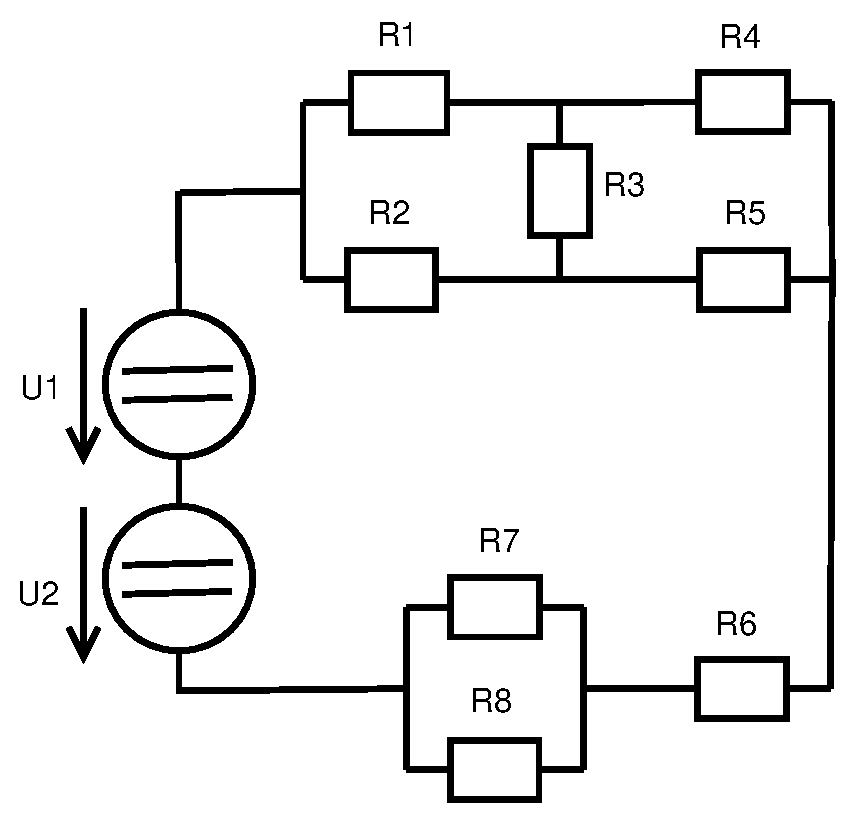
\includegraphics[scale=0.4]{pr1/Diagram1.eps}
    \\
\end{tabular}


\vspace{1mm}
\begin{tabular}{|c|c|c|c|c|c|c|c|c|c|c|}
    \hline
     & $U_1 [V]$ &$ U_2 [V] $& $R_1[\Omega] $&$ R_2[\Omega] $&$ R_3[\Omega] $&$ R_4[\Omega] $&$ R_5[\Omega] $&$ R_6[\Omega] $&$ R_7[\Omega] $&$ R_8 [\Omega] $
     \\
     \hline
    H & 135 & 80 & 680 & 600 & 260 & 310 & 575 & 8702 & 355 & 265  
    \\
    \hline
\end{tabular}
\vspace{1mm}
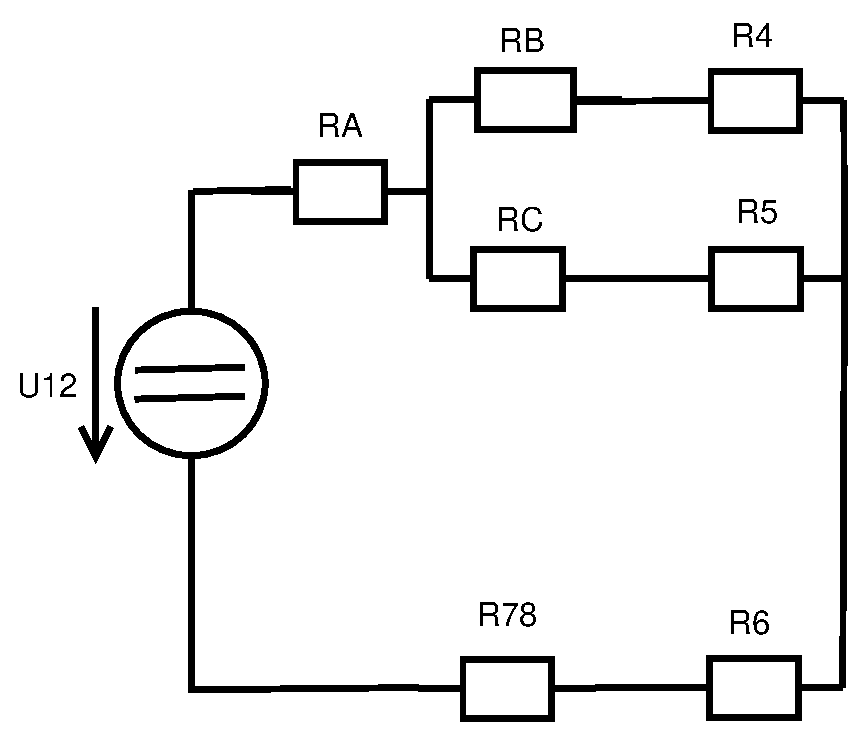
\includegraphics[scale=0.4]{pr1/Diagram2.eps}

Postupně zjednodušíme celý obvod.

$$ U_{12} = U_1 + U_2 = 135 + 80 = 215 V $$
\vspace{1mm}
$$ R_{87} = \frac{R_7 * R_8}{R_7 + R_8} = \frac{355 * 265}{355 + 265} = \frac{18815}{124} \Omega $$
\vspace{1mm}
$$ R_A = \frac{R_1 * R_2}{R_1 + R_2 + R_3} = \frac{680 * 600}{680 + 600 +260} = \frac{20400}{77}\Omega $$
\vspace{1mm}
$$ R_B = \frac{R_1 * R_3}{R_1 + R_2 + R_3} = \frac{680 * 260}{680 + 600 +260} = \frac{8840}{77}\Omega $$
\vspace{1mm}
$$ R_C = \frac{R_2 * R_3}{R_1 + R_2 + R_3} = \frac{600 * 260}{680 + 600 +260} = \frac{7800}{77}\Omega $$
\vspace{1mm}

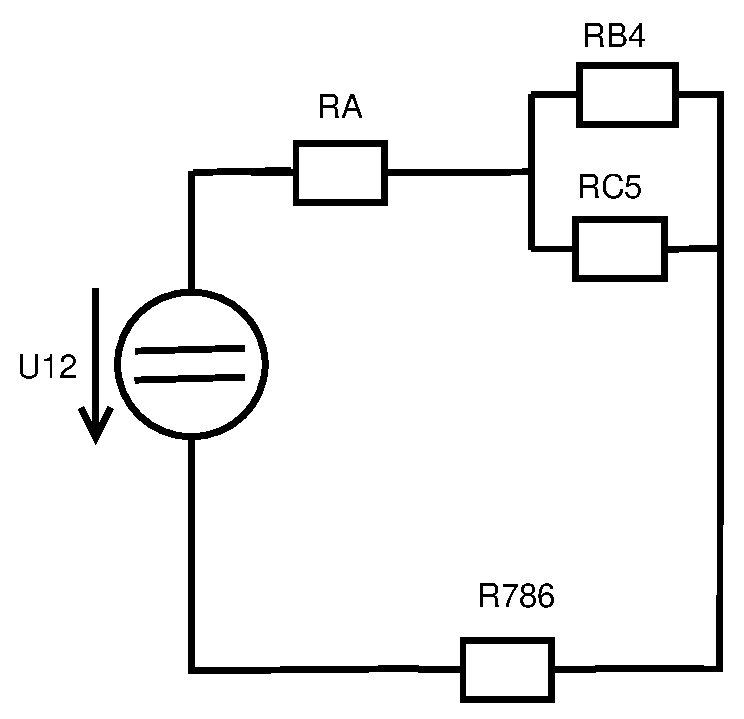
\includegraphics[scale=0.4]{pr1/Diagram3.eps}

$$ R_{786} = R_{78} + R_6 = \frac{18815}{124} + 870 = 1021.7338 \Omega $$
\vspace{1mm}
$$ R_{B4} = R_B + R_4 = \frac{8840}{77} + 310 = \frac{32710}{77} = 424.8052 \Omega $$
\vspace{1mm}
$$ R_{C5} = R_C + R_5 = \frac{7800}{77} + 575 = \frac{52075}{77} = 676.2987 \Omega $$
\vspace{1mm}

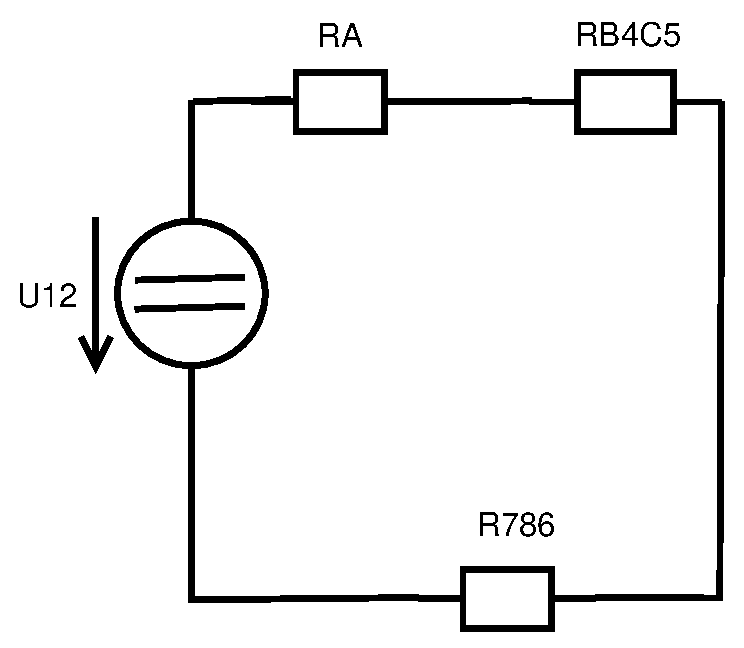
\includegraphics[scale=0.4]{pr1/Diagram4.eps}

$$ R_{B4C5} = \frac{R_{B4} * R_{C5}}{R_{B4} + R_{C5}} = \frac{424.8052 * 676.2987}{424.8052 + 676.2987} = 382.8282 \Omega $$
\vspace{1mm}

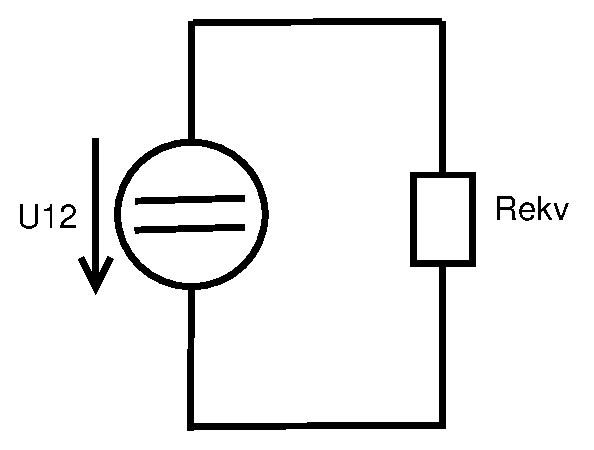
\includegraphics[scale=0.4]{pr1/Diagram5.eps}

$$ R_{ekv} = R_A + R_{B4C5} + R_{786} = \frac{20400}{77} + 382.8282 = 1669.4971 \Omega $$
\vspace{3mm}

Teď vypočítáme proud tekoucí zjednodušeným obvodem.
$$ I = \frac{U_{12}}{R_{ekv}} = \frac{215}{1669.4971} = 0.1288 A$$
\vspace{1mm}
Máme proud celkový proud tekoucí obvodem, takže se budeme postupně vracet a dopočítávat jednotlivá napětí a proudy.
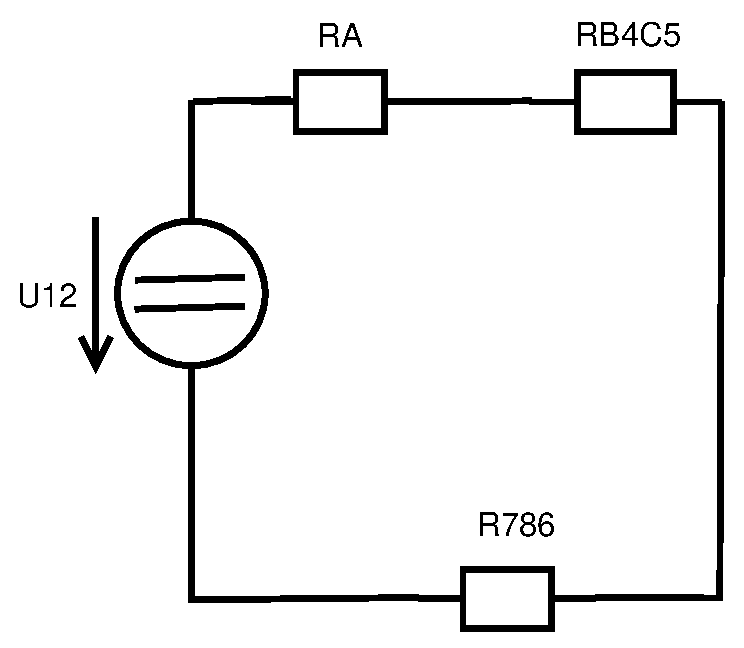
\includegraphics[scale=0.4]{pr1/Diagram4.eps}
\vspace{1mm}
$$ U_{RA} = R_A * I = \frac{20400}{77} * 0.1288 = 34.1236V $$
\vspace{1mm}
$$ U_{RB4C5} = R_{B4C5} * I = 382.8282 * 0.1288 = 49.3083V $$
\vspace{1mm}
$$ U_{R786} = R_{786} * I = 1021.7338 * 0.1288 = 131.5993 V $$
\vspace{1mm}
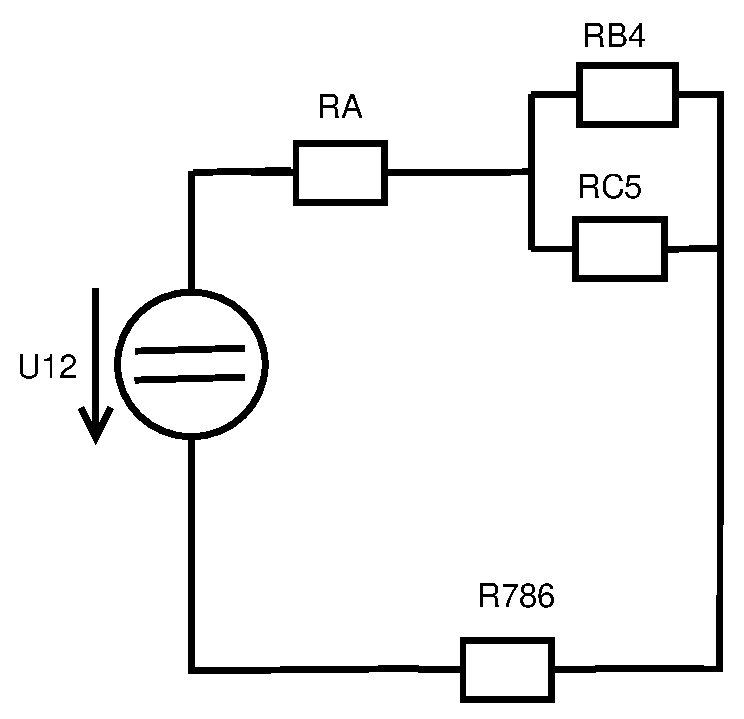
\includegraphics[scale=0.4]{pr1/Diagram3.eps}
\vspace{1mm}
$$ I_{RB4} = \frac{U_{RB4C5}}{R_{B4}} = \frac{49.3083}{424.8052} = 0.1161 A $$
\vspace{1mm}
$$ I_{RC5} = \frac{U_{RB4C5}}{R_{C5}} = \frac{49.3083}{676.2987} = 0.0729 A $$
\vspace{1mm}

\newpage
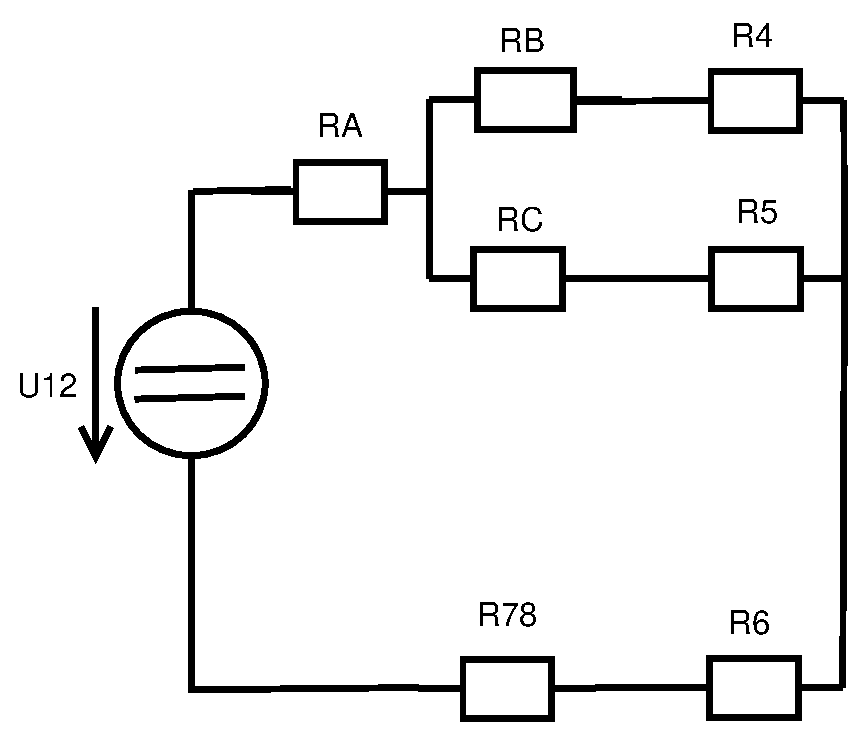
\includegraphics[scale=0.4]{pr1/Diagram2.eps}
\vspace{1mm}
$$ U_{RB} = R_B * I_{RB4} = \frac{8840}{77} * 0.1161 = 13.3289 V $$
\vspace{1mm}
$$ U_{R4} = R_4 * I_{RB4} = 310 * 01161 = 35.9910 V $$
\vspace{1mm}
$$ U_{RC} = R_C * I_{RC5} = \frac{7800}{77} * 0.0729 = 7.3847 V$$
\vspace{1mm}
$$ U_{R5} = R_5 * I_{RC5} =  575 * 0.0729 = 41.9175 V$$
\vspace{1mm}
$$ U_{R6} = I * R_6 = 0.1288 * 870 = 112.056 V $$
\vspace{1mm}
$$ U_{R78} = I * R_{78} = 0.1288 * \frac{18815}{124} = 19.5433 V $$
\vspace{1mm}
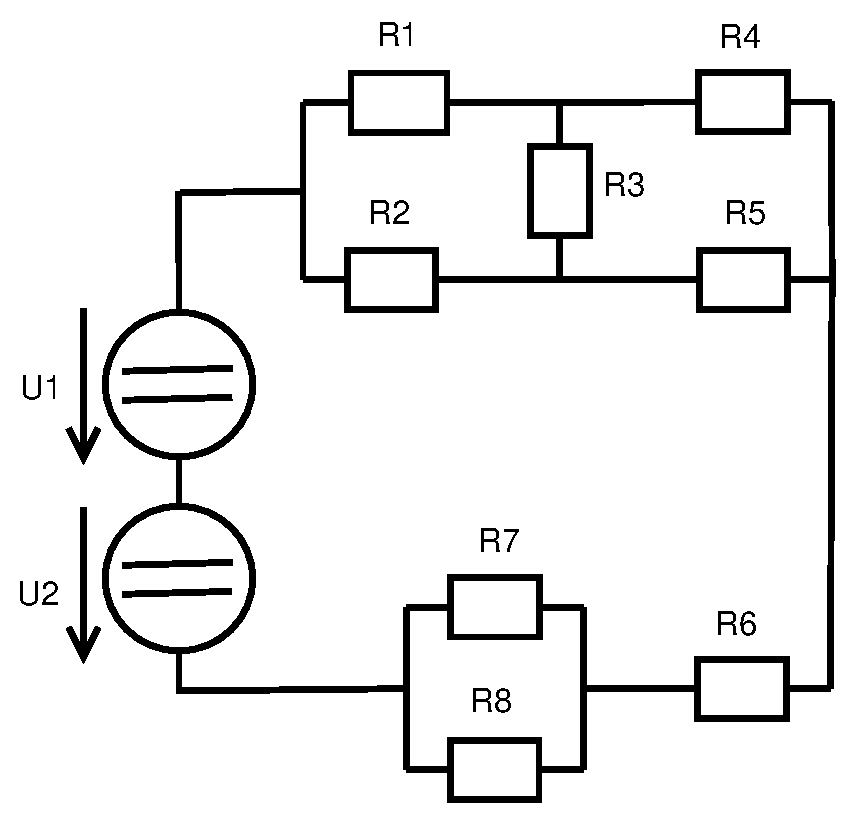
\includegraphics[scale=0.4]{pr1/Diagram1.eps}
\vspace{1mm}
$$ I_{R7} = \frac{U_{R78}}{R_7} = \frac{19.5433}{355} = 0.0551 A $$
\vspace{1mm}
$$ I_{R8} = \frac{U_{R78}}{R_8} = \frac{19.5433}{265} = 0.0737 A $$
\vspace{1mm}
$$ U_{R8} = U_{R78} = 19.5433 V $$

\newpage
\section{Příklad č.2}

\begin{tabular}{c c}
    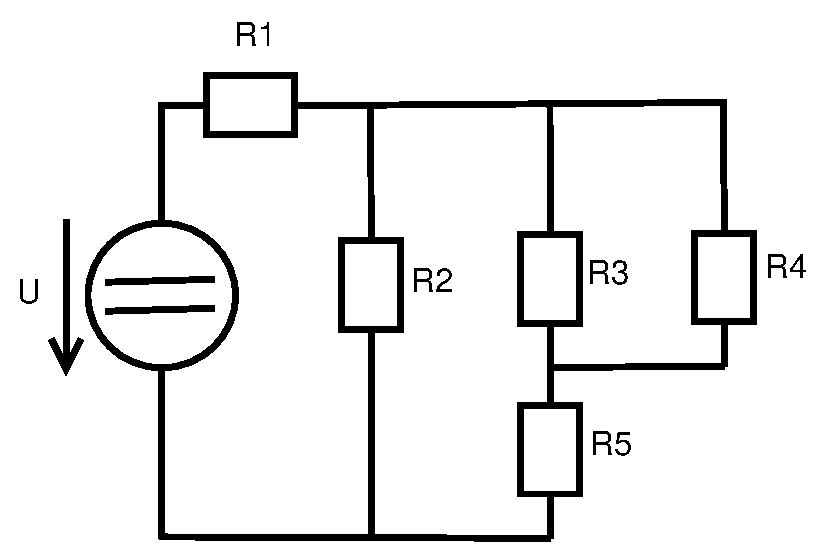
\includegraphics[scale=0.5]{pr2/bb_1.eps}
    &
    \begin{minipage}{7cm}
        .\\[-5cm]
        Stanovte napětí $U_{R4}$ a proud $I_{R4}$. Použijte metodu Théveninovy věty.
    \end{minipage}
\end{tabular}

\begin{tabular}{|c|c|c|c|c|c|c|}
    \hline
    & $U [V]$ & $R_1 [\Omega]$ & $R_2 [\Omega]$ & $R_3 [\Omega]$ & $R_4 [\Omega]$ & $R_5 [\Omega]$
    \\ \hline
    C & 200 & 220 & 630 & 240 & 450 & 230
    \\ \hline
\end{tabular}
\vspace{1mm}

Zapojíme $R_4$ do náhradního obvodu a vyjádříme rovnici pro proud $I_{R4}$.

\begin{tabular}{ c c }
    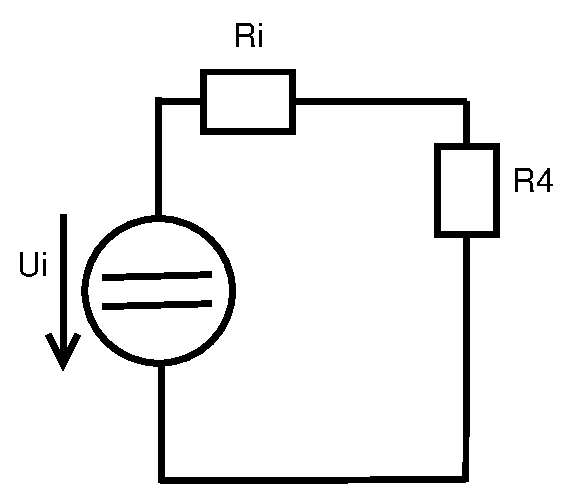
\includegraphics[scale=0.5]{pr2/bb_2.eps}
    &
    \begin{minipage}{4cm}
        .\\[-4cm]
        $$ I_{R4} = \frac{U_i}{R_i + R_4} $$
    \end{minipage}
\end{tabular}
\vspace{3mm}

Vyjádříme si $R_i$, které následně i vypočteme. 
\\[5mm]
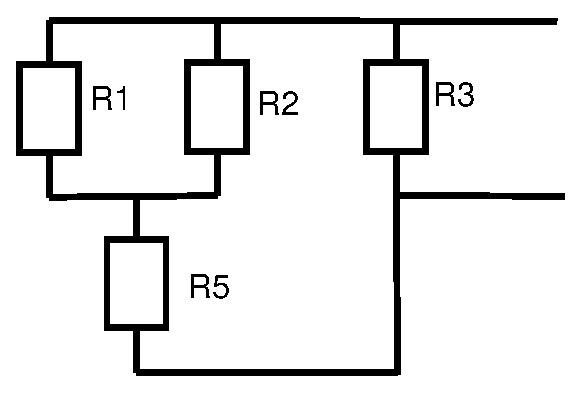
\includegraphics[scale=0.5]{pr2/bb_3.eps}
\vspace{1mm}
$$ R_{12} = \frac{R_1 * R_2}{R_1 + R_2} = \frac{220 * 630}{220 + 630} = \frac{2772}{17} \Omega $$
\vspace{1mm}
$$ R_{125} = R_5 + R_{12} = 230 + \frac{2772}{17} = \frac{6682}{17} \Omega$$
\vspace{1mm}
$$ R_i = \frac{R_{125} * R_3}{R_{125} + R_3} = \frac{6682/17 * 240}{6682/17 + 240} = 149.0132 \Omega $$

\newpage

$R_i$ máme a teď ještě potřebujeme $U_i$. $U_i$ je schodné s napětím na rezistoru $R_3$.  

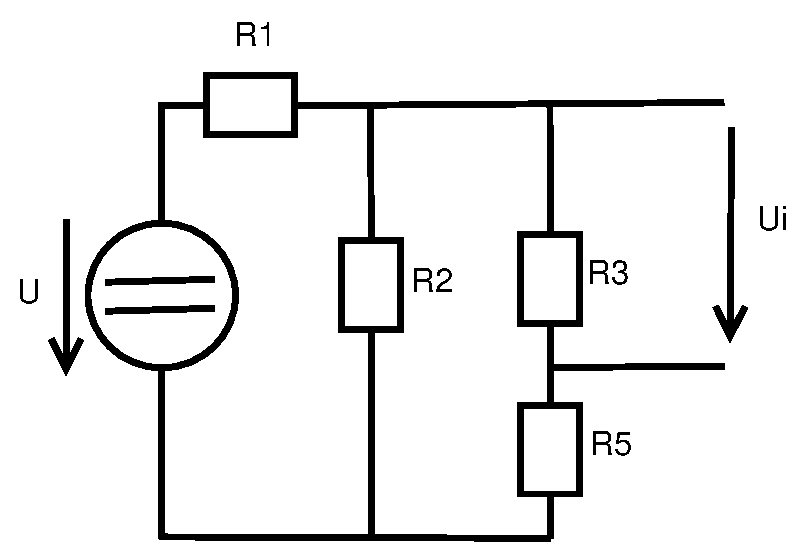
\includegraphics[scale=0.5]{pr2/bb_4.eps}
\vspace{1mm}
$$ I_x * R_1 + I_x * R_3 + I_x * R_5 - U = 0 $$
$$ I_x*(R_1 + R_2 + R_3) = U $$
$$ I_x = \frac{U}{R_1 + R_2 + R_3} = \frac{200}{220+240+230} = \frac{200}{690} = \frac{20}{69} A$$
\vspace{3mm}
$$ U_i = U_{R3} $$
\vspace{1mm}
$$ U_i = I_x * R_3 = \frac{20}{69} * 630 = 182.6087 V $$
\vspace{3mm}
Když už máme $R_i$ i $U_i$ můžeme dosadit do rovnice a vypočítat $I_{R4}$ a následně i $U_{R4}$.
$$ I_{R4} = \frac{U_i}{R_i+R_4} = \frac{182.6087}{149.0132 + 450} = 0.3048 A $$
\vspace{1mm}
$$ U_{R4} = I_{R4} * R_4 = 0.3048 * 450 = 137.16 V $$


\newpage
\section{Příklad č.3}

Stanovte napětí $U_{R4}$ a proud $I_{R4}$. Použijte metodu uzlových napětí ($U_a, U_b, U_c$).

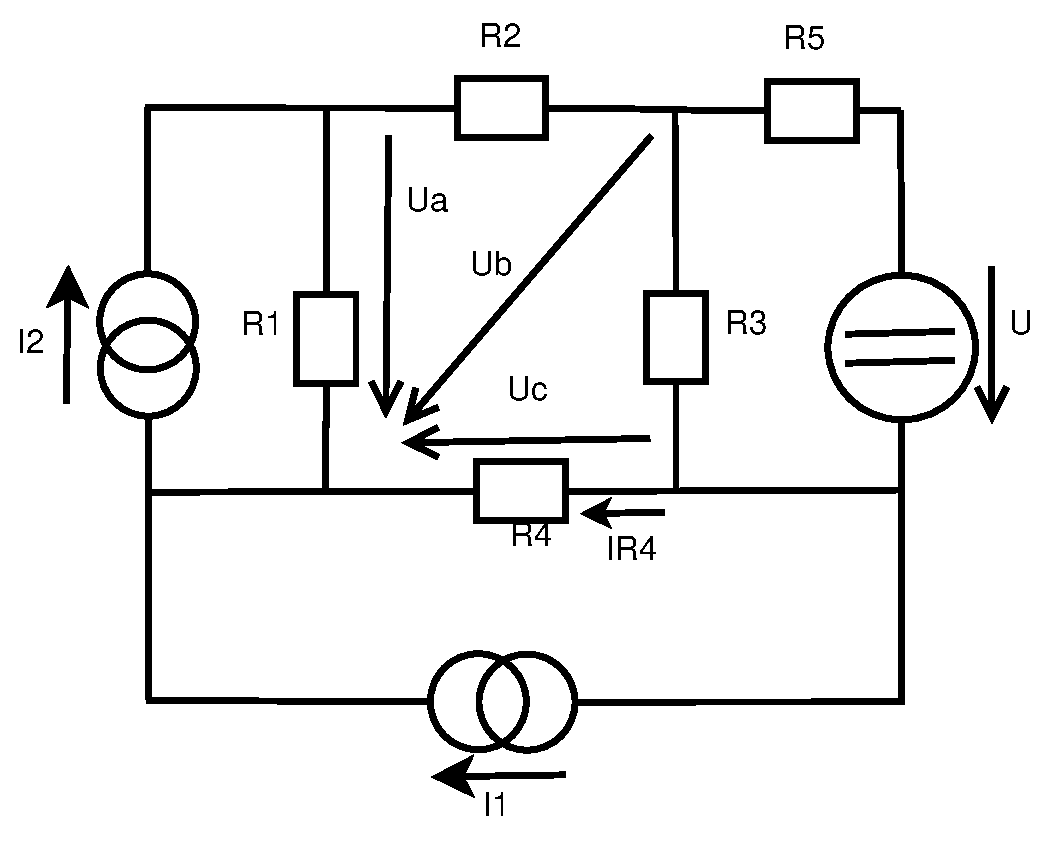
\includegraphics[scale=0.5]{pr3/cc_01.eps}

\begin{tabular}{|c|c|c|c|c|c|c|c|c|}
    \hline
    sk. &$ U[V] $&$ I_1[A] $&$ I_2[A] $&$ R_1[\Omega] $&$ R_2[\Omega] $&$ R_3[\Omega] $&$ R_4[\Omega] $&$ R_5[\Omega] $
    \\ \hline
    A & 120 & 0.9 & 0.7 & 53 & 49 & 65 & 39 & 32
    \\ \hline
\end{tabular}
\\
\vspace{3mm}
Nejdříve si určíme uzly a směry proudů.\\

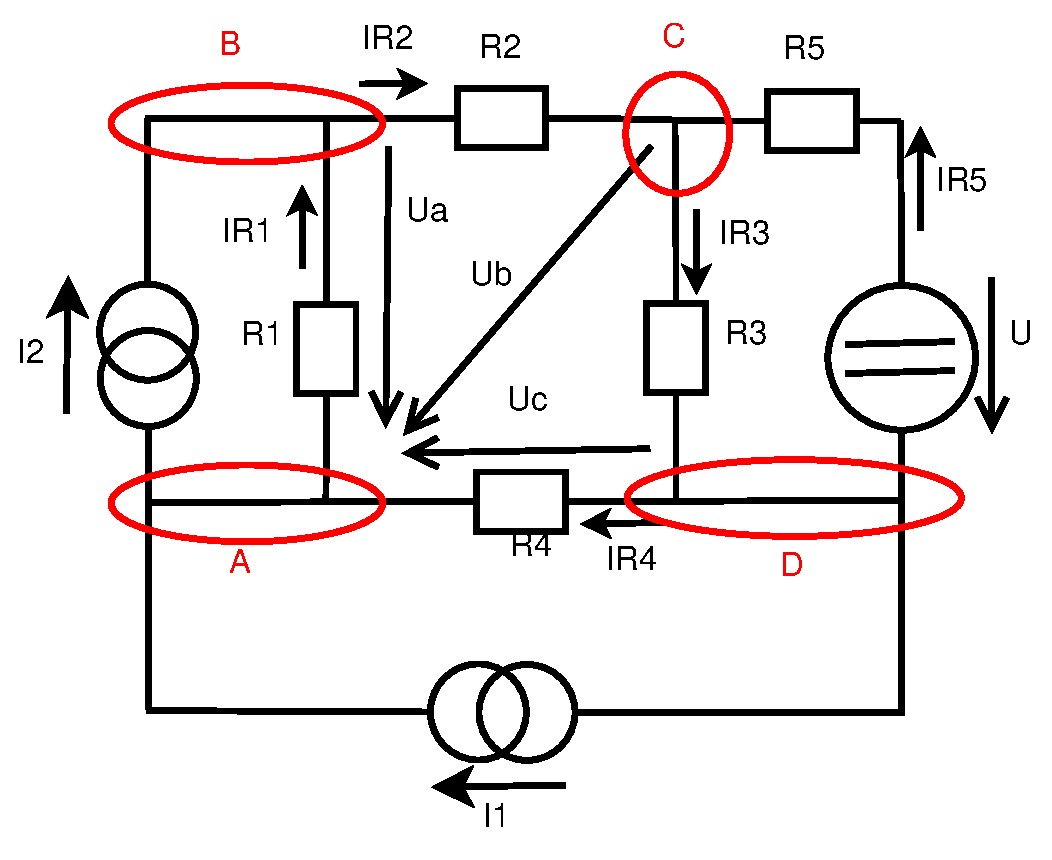
\includegraphics[scale=0.5]{pr3/cc_02.eps}

Podle 1.Kirchhoffova zákona sestrojíme rovnice pro uzly B, C a D. 
$$ B: I_2 + I_{R1} - I_{R2} = 0 $$
$$ C: I_{R2} + I_{R5} - I_{R3} = 0 $$
$$ D: I_{R3} - I_{R4} - I_{R5} - I_1 = 0 $$
Teď rozložíme schéma zapojení a určíme rovnice pro jednotlivé proudy.

\begin{tabular}{|c|c|c|}
    \hline
    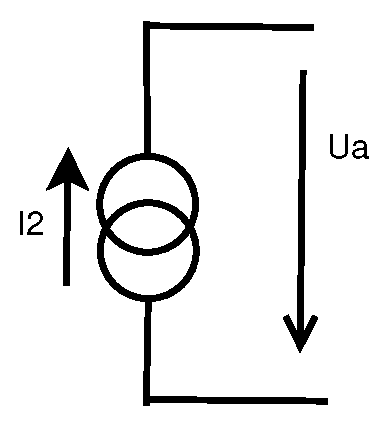
\includegraphics[scale=0.5]{pr3/cc_11.eps}
    & 
    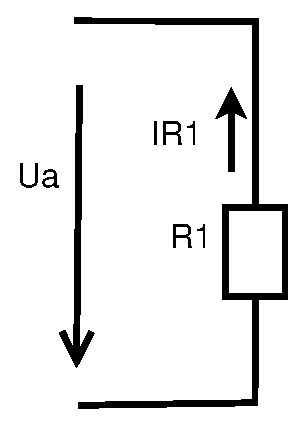
\includegraphics[scale=0.5]{pr3/cc_12.eps}
    & 
    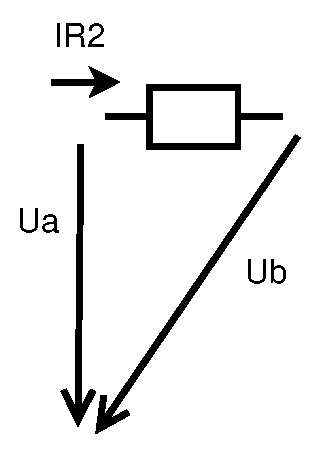
\includegraphics[scale=0.5]{pr3/cc_13.eps}
    \\
    \hline
    \begin{minipage}{5cm}
        $I_2 = I_2 = 0.7A$
    \end{minipage}
    &
    \begin{minipage}{5cm}
        $$ I_{R1}R_1 + U_a = 0 $$
        $$ I_{R1} = \frac{-U_a}{ R_1} $$
    \end{minipage}
    &
    \begin{minipage}{5cm}
        $$ I_{R2}R2 + U_b - U_a = 0 $$
        $$ I_{R2} = \frac{U_a - U_b}{R_2} $$
    \end{minipage}
    
    \\
    \hline
    
    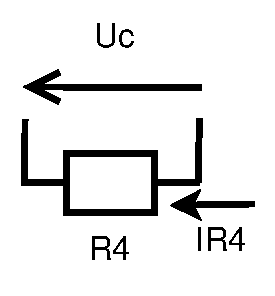
\includegraphics[scale=0.5]{pr3/cc_14.eps}
    & 
    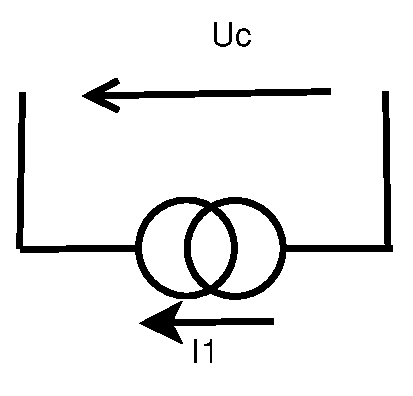
\includegraphics[scale=0.5]{pr3/cc_15.eps}
    & 
    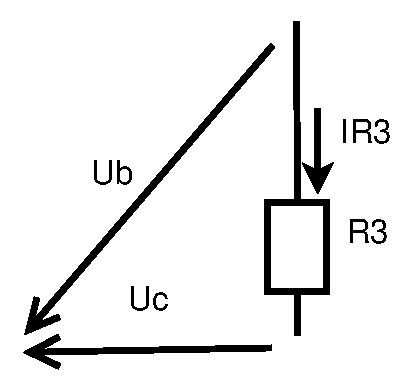
\includegraphics[scale=0.5]{pr3/cc_16.eps}
    \\
    \hline
    \begin{minipage}{5cm}
        $$ I_{R4}R4 - U_c = 0 $$
        $$ I_{R4} = \frac{U_c}{R_4} $$
    \end{minipage}
    &
    \begin{minipage}{5cm}
        $$ I_1 = I_1 = 0.9A $$
    \end{minipage}
    &
    \begin{minipage}{5cm}
        $$ I_{R3}R3 + U_c - U_b = 0 $$
        $$ I_{R3} = \frac{U_b - U_c}{R_3} $$
    \end{minipage}
    
    \\
    \hline
    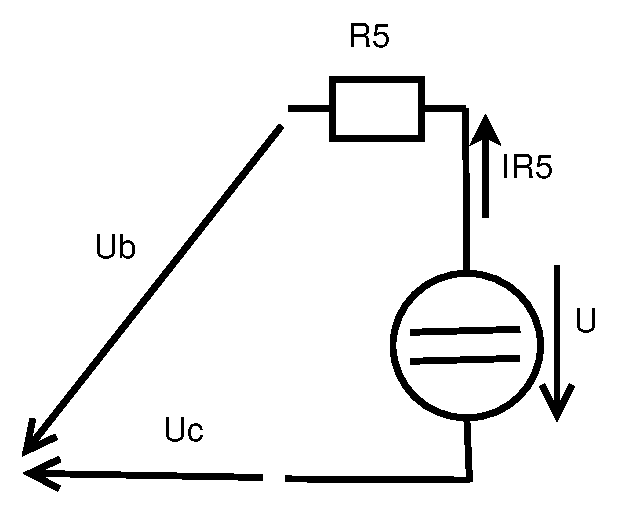
\includegraphics[scale=0.5]{pr3/cc_17.eps}
    &
    \multicolumn{2}{c|}
    {
        \begin{minipage}{5cm}
            $$ I_{R5}R5 + U_b - U_c - U = 0 $$
            $$ I_{R5} = \frac{U + U_c - U_b}{R_5} $$
            \\
            \\
        \end{minipage}
    }
    \\
    \hline
\end{tabular}
\\[5mm]
Dosadíme proudy do rovnic uzlů.
$$ B: I_2 + \frac{-U_a}{R_1} - \frac{U_a -U_b}{R_2} = 0 $$
$$ C: \frac{U_a - U_b}{R2} +\frac{U+U_c-U_b}{R_5} - \frac{U_b-U_c}{R_3} = 0 $$
$$ D: \frac{U_b - U_c}{R_3} - \frac{U_c}{R_4} - \frac{U + U_c - U_b}{R_5}= 0 $$
\\
\newpage
Z rovnice B si vyjádříme $U_a$.
$$ B: I_2 + \frac{-U_a}{R_1} - \frac{U_a -U_b}{R_2} = 0 $$
$$ I_2R_1R_2 - U_aR_2 -U_aR1 + U_bR_1 = 0 $$
$$ I_2R_1R_2 + U_bR_1 = U_aR_2 +U_aR1 $$
$$ I_2R_1R_2 + U_bR_1 = U_a(R_2 +R_1) $$
$$ U_a = \frac{I_2R_1R_2 + U_bR_1}{R_1 + R_2} $$
\\
Do rovnice C dosadíme $U_a$ a vyjádříme si $U_b$.
$$ C: \frac{U_a - U_b}{R2} +\frac{U+U_c-U_b}{R_5} - \frac{U_b-U_c}{R_3} = 0 $$
$$ \frac{\frac{I_2R_1R_2 + U_bR_1}{R_1 + R_2} - U_b}{R2} +\frac{U+U_c-U_b}{R_5} - \frac{U_b-U_c}{R_3} = 0 $$
$$ \frac{I_2R_1R_2 + U_bR_1}{R_1 + R_2}R_3R_5 - U_bR_3R_5 +UR_2R_3 + U_cR_2R_3 - U_bR_2R_3 - U_bR_2R_5 + U_cR_2R_5 = 0 $$
$$ \frac{I_2R_1R_2 + U_bR_1}{R_1 + R_2}R_3R_5 +UR_2R_3 + U_cR_2R_3 + U_cR_2R_5 = U_bR_3R_5 + U_bR_2R_3 + U_bR_2R_5 $$

$$ I_2R_1R_2R_3R_5 + U_bR_1R_3R_5 + (R_1 + R_2)(UR_2R_3 + U_cR_2R_3 + U_cR_2R_5) = $$
$$ = U_bR_1R_3R_5 + U_bR_2R_3R_5 + U_bR_1R_2R_3 + U_bR_2R_2R_3 + U_bR_1R_2R_5 + U_bR_2R_2R_5 $$

$$ I_2R_1R_2R_3R_5 + (R_1 + R_2)(UR_2R_3 + U_cR_2R_3 + U_cR_2R_5) = $$
$$ = U_bR_1R_3R_5 + U_bR_2R_3R_5 + U_bR_1R_2R_3 + U_bR_2R_2R_3 + U_bR_1R_2R_5 + U_bR_2R_2R_5 -U_bR_1R_3R_5 $$

$$ I_2R_1R_2R_3R_5 + (R_1 + R_2)(UR_2R_3 + U_cR_2R_3 + U_cR_2R_5) = $$
$$ = U_b (R_1R_3R_5 + R_2R_3R_5 + R_1R_2R_3 + R_2R_2R_3 + R_1R_2R_5 + R_2R_2R_5 -R_1R_3R_5) $$

$$ \frac{I_2R_1R_2R_3R_5 + (R_1 + R_2)(UR_2R_3 + U_cR_2R_3 + U_cR_2R_5)}{R_1R_3R_5 + R_2R_3R_5 + R_1R_2R_3 + R_2R_2R_3 + R_1R_2R_5 + R_2R_2R_5 -R_1R_3R_5} = U_b $$

$$ \frac{I_2R_1R_2R_3R_5 + (R_1 + R_2)(UR_2R_3 + U_cR_2R_3 + U_cR_2R_5)}{R_3R_5 (R_1 + R_2) + R_2R_3 (R_1 +R_2) + R_2R_5 + (R_1 + R_2) -R_1R_3R_5} = U_b $$

\newpage
Dosadíme $U_b$ do rovnice uzlu D.

$$ D: \frac{U_b - U_c}{R_3} - \frac{U_c}{R_4} - \frac{U + U_c - U_b}{R_5}= 0 $$

$$ \frac{\frac{I_2R_1R_2R_3R_5 + (R_1 + R_2)(UR_2R_3 + U_cR_2R_3 + U_cR_2R_5)}{R_3R_5 (R_1 + R_2) + R_2R_3 (R_1 +R_2) + R_2R_5 + (R_1 + R_2) -R_1R_3R_5} - U_c}{R_3} - \frac{U_c}{R_4} - $$
$$ - \frac{U + U_c - \frac{I_2R_1R_2R_3R_5 + (R_1 + R_2)(UR_2R_3 + U_cR_2R_3 + U_cR_2R_5)}{R_3R_5 (R_1 + R_2) + R_2R_3 (R_1 +R_2) + R_2R_5 + (R_1 + R_2) -R_1R_3R_5}}{R_5}= 0 $$

Dosadíme hodnoty a vypočítáme $U_c$.

$$ \frac{\frac{0.7*53*49*65*32 + (53 + 49)(120*49*65 + U_c*49*65 + U_c*49*32)}{65*32 (53 + 49) + 49*65 (53 +49) + 49*32 + (53 + 49) -53*65*32} - U_c}{65} - \frac{U_c}{39} - $$
$$ - \frac{120 + U_c - \frac{0.7*53*49*65*32 + (53 + 49)(120*49*65 + U_c*49*65 + U_c*49*32)}{65*32 (53 + 49) + 49*65 (53 +49) + 49*32 + (53 + 49) -53*65*32}}{32}= 0 $$

$$ \frac{ \frac{ 3781232 + 102(382200+4753U_c) }{ 2080*102+3185*102+1568*102-110240 }-U_c }{65} - \frac{U_c}{39} - \frac{120 + U_c - \frac{ 3781232 + 102(382200+4753U_c) }{ 2080*102+3185*102+1568*102-110240 }}{32} = 0 $$

$$ \frac{ \frac{42765632 + 484806U_c}{586726} - U_c}{65} - \frac{U_c}{39} - \frac{120 + U_c - \frac{42765632 + 484806U_c}{586726} }{32} = 0 $$

$$ \frac{72.8889+0.8263U_c - U_c}{65} - \frac{U_c}{39} - \frac{120 + U_c -72.8889 - 0.8263U_c}{32} = 0 $$

$$ 90965.3472+1031.2224U_c-1248U_c-2080U_c-304200-2535U_c+184773.3615+2094.6705U_c = 0 $$

$$ -28461.2913 - 2737.1071U_c = 0 $$

$$ -28461.2913 = 2737.1071U_c $$

$$ -10.3983 = U_c $$

$$ U_c = -10.3983 V $$

Máme $U_c$, takže ho můžeme dosadit do rovnice pro výpočet $I_{R4}$.

$$ I_{R4} = \frac{U_c}{R_4} = \frac{-10.3983}{39} = -0.2666A $$

Proud $I_{R4}$ vyšel záporný. To znamená, že je opačného směru než jsme předpokádali. Ještě dopočítáme $U_{R4}$.

$$ U_{R4} = I_{R4} * R_4 = -0.2666 * 39 = -10.3974 V $$



\newpage
\section{Příklad č.4}
\begin{tabular}{c c}
    \begin{minipage}{8cm}
        .\\[-6cm]
        Pro napájecí napětí platí: \\
        $u_1 = U_1 * \sin (2\pi ft), u_2 = U_2 * \sin (2\pi ft)$.
        \\
        Ve vyztahu pro napětí $u_{C1} = U_{C1} * \sin (2\pi ft + \varphi_{C_1})$ určete $|U_{C1}|$ a $\varphi_{C1}$. Použijte metodu smyčkových proudů.
        \\
        \\
        Pozn: Pomocné "směry šipek napájecích zdrojů platí pro speciální časový okamžik $ (t = \frac{\pi}{2\omega}) $."
    \end{minipage}
    &
    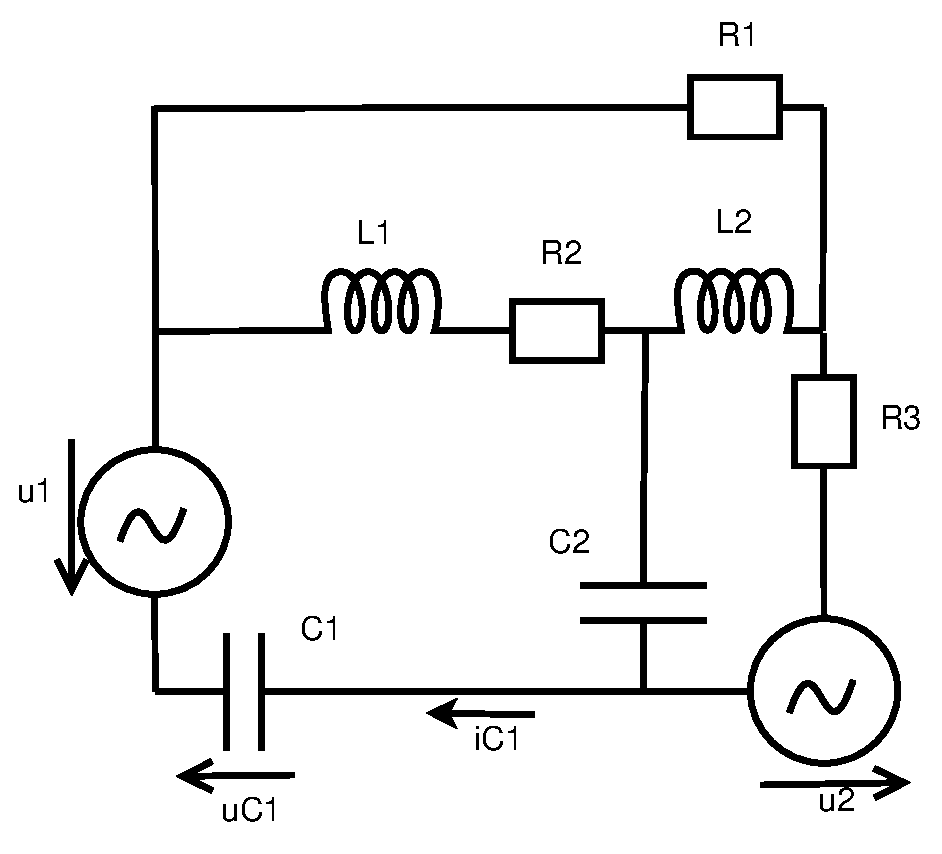
\includegraphics[scale=0.5]{pr4/dd_1.eps}
\end{tabular}
\\
\begin{tabular}{|c|c|c|c|c|c|c|c|c|c|c|}
    \hline
    sk &$ U_1[V] $&$ U_2[V] $&$ R_1[\Omega] $&$ R_2[\Omega] $&$ R_3[\Omega] $&$ L_1[mH] $&$ L_2[mH] $&$ C[\mu F] $&$ C[\mu F] $&$ f[Hz] $
    
    \\ \hline
    H & 65 & 60 & 10 & 10 & 12 & 160 & 75 & 155 & 70 & 95
    \\ \hline
\end{tabular}
\\
 ...
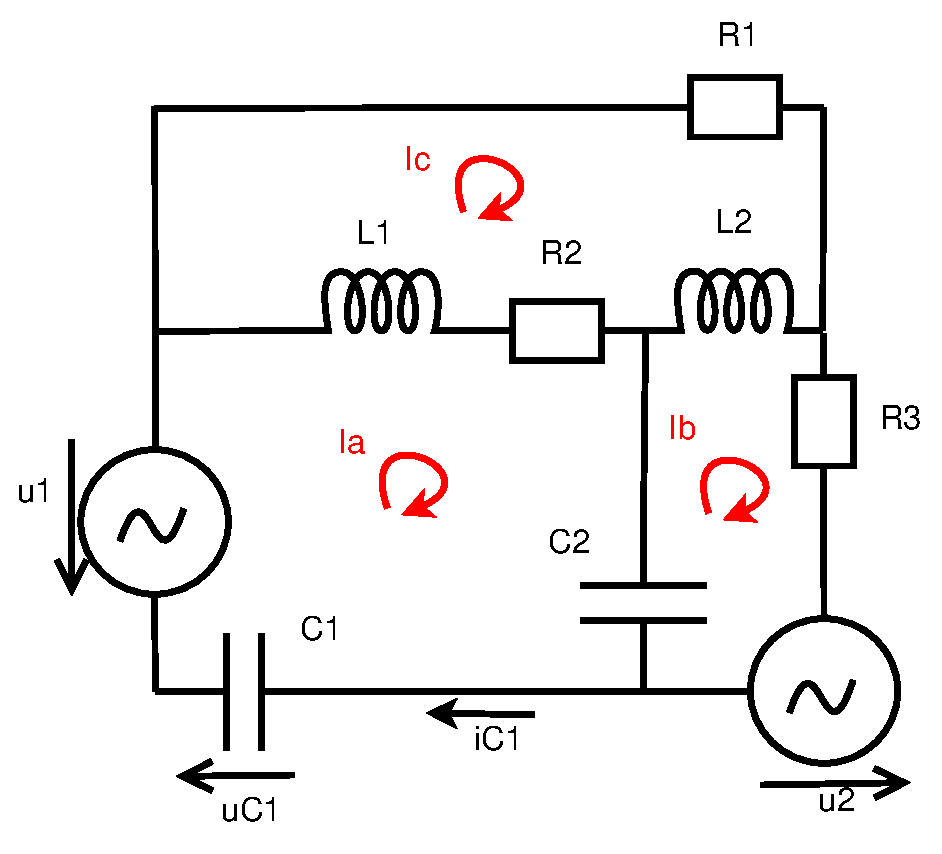
\includegraphics[scale=0.5]{pr4/dd_2.eps}
 ...
 \newpage
\section{Příklad č.5}

\begin{tabular}{c c}
    \begin{minipage}{8cm}
        .\\[-4cm]
        Sestrojete diferenciální rovnici popisující chování obvodu na obrázku, dále ji upravte dosazením hodnot parametrů. Vypočítejte analytické řešení $i_L = f(t)$. Proveďte kontrolu dosazením do sestavené diferenciální rovnice.
    \end{minipage}
    &
    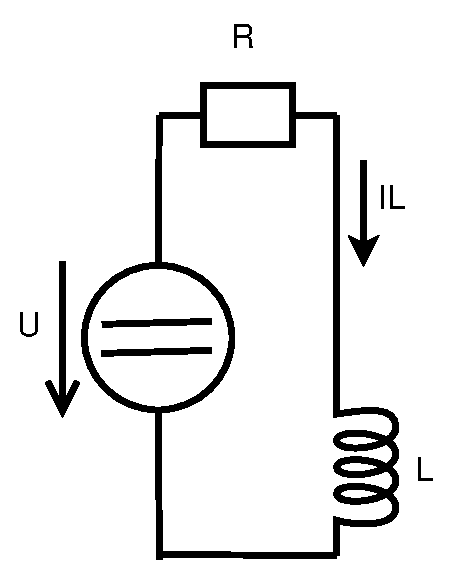
\includegraphics[scale=0.5]{pr5/ee_1.eps}
\end{tabular}
\\
\begin{tabular}{|c|c|c|c|c|}
    \hline
    sk &$ U[V] $&$ L[H] $&$ R[\Omega] $&$ i_L[A] $
    \\ \hline
    C & 60 & 5 & 30 & 7 
    \\ \hline
\end{tabular}

$$ $$
Mějmě základní diferenciální rovnici pro výpočet proudu $i'_L$.
$$ i'_L = \frac{1}{L} * u_L $$

Jelikož neznáme $u_L$, tak si ho vyjádříme za pomoci II.Kirchhoffova zákonu.
$$ i_LR + u_L - U = 0 $$
$$ u_L = U - i_LR $$

Teď $u_L$ dosadíme a získáme konečnou podobu naší diferenciální rovnice.
$$ i'_L = \frac{1}{L}*(U -i_LR) $$


$$ i'_L = \frac{1}{5}*(60-i_L*30) $$
$$ i'_L = 12 - 6i_L $$
...

\newpage
\section{Závěr}

\begin{tabular}{|c|c|c|c|}
    \hline
    Př. & Sk & \multicolumn{2}{|c|}{}
    \\ \hline
    \multicolumn{2}{|c|}{} & $\mathbf{U_{R8}}$ & $\mathbf{I_{R8}}$
    \\ \hline
    1 & H & $19.5433V$ & $0.0737A$
    \\ \hline
    \multicolumn{2}{|c|}{} & $\mathbf{U_{R4}}$ & $\mathbf{I_{R4}}$
    \\ \hline
    2 & C & $137.16V$ & $0.3048A$
    \\ \hline
    \multicolumn{2}{|c|}{} & $\mathbf{U_{R4}}$ & $\mathbf{I_{R4}}$
    \\ \hline
    3 & A & $-10.3974V$ & $-0.2666A$
    \\ \hline
    \multicolumn{2}{|c|}{} &  & 
    \\ \hline
    4 & H &  & 
    \\ \hline
    \multicolumn{2}{|c|}{} &  & 
    \\ \hline
    5 & C &  & 
    
    \\ \hline
\end{tabular}


\end{document}
